% final draft
% todo: Interkapitel-Referenzen, Kontextgrafik

\chapter{Mentale Modelle} % (fold)
\label{cha:mentale_modelle}

In diesem Kapitel wird das Konzept der \emph{„mentalen Modelle“} eingeführt, das in dieser Arbeit als Erklärungsansatz für jene Aspekte von „Articulation Work“ verwendet wird, die die nicht sichtbaren, kognitiven Beiträge eines beteiligten Individuums betreffen. Nach einer Einführung in die Begriffswelt der mentalen Modelle wird die Argumentation aus dem Kapitel „Articulation Work“ nochmals aufgegriffen und die mögliche Rolle mentaler Modelle für die Durchführung derselben erörtert. In der Folge werden Methoden eingeführt, mit denen mentale Modelle externalisiert und kommuniziert werden können. Basierend auf diesen Beschreibungen wird im letzten Teil des Kapitels untersucht, welche Herausforderungen sich bei der Anwendung dieser Methoden im Kontext von „Articulation Work“ ergeben können. Abbildung \ref{fig:img_Kontextgrafiken_k3} stellt dieses Kapitel und dessen Aufbau im Kontext der anderen inhaltlich vor- und nachgelagerten Kapitel dar.


\begin{figure}[htbp]
	\centering
		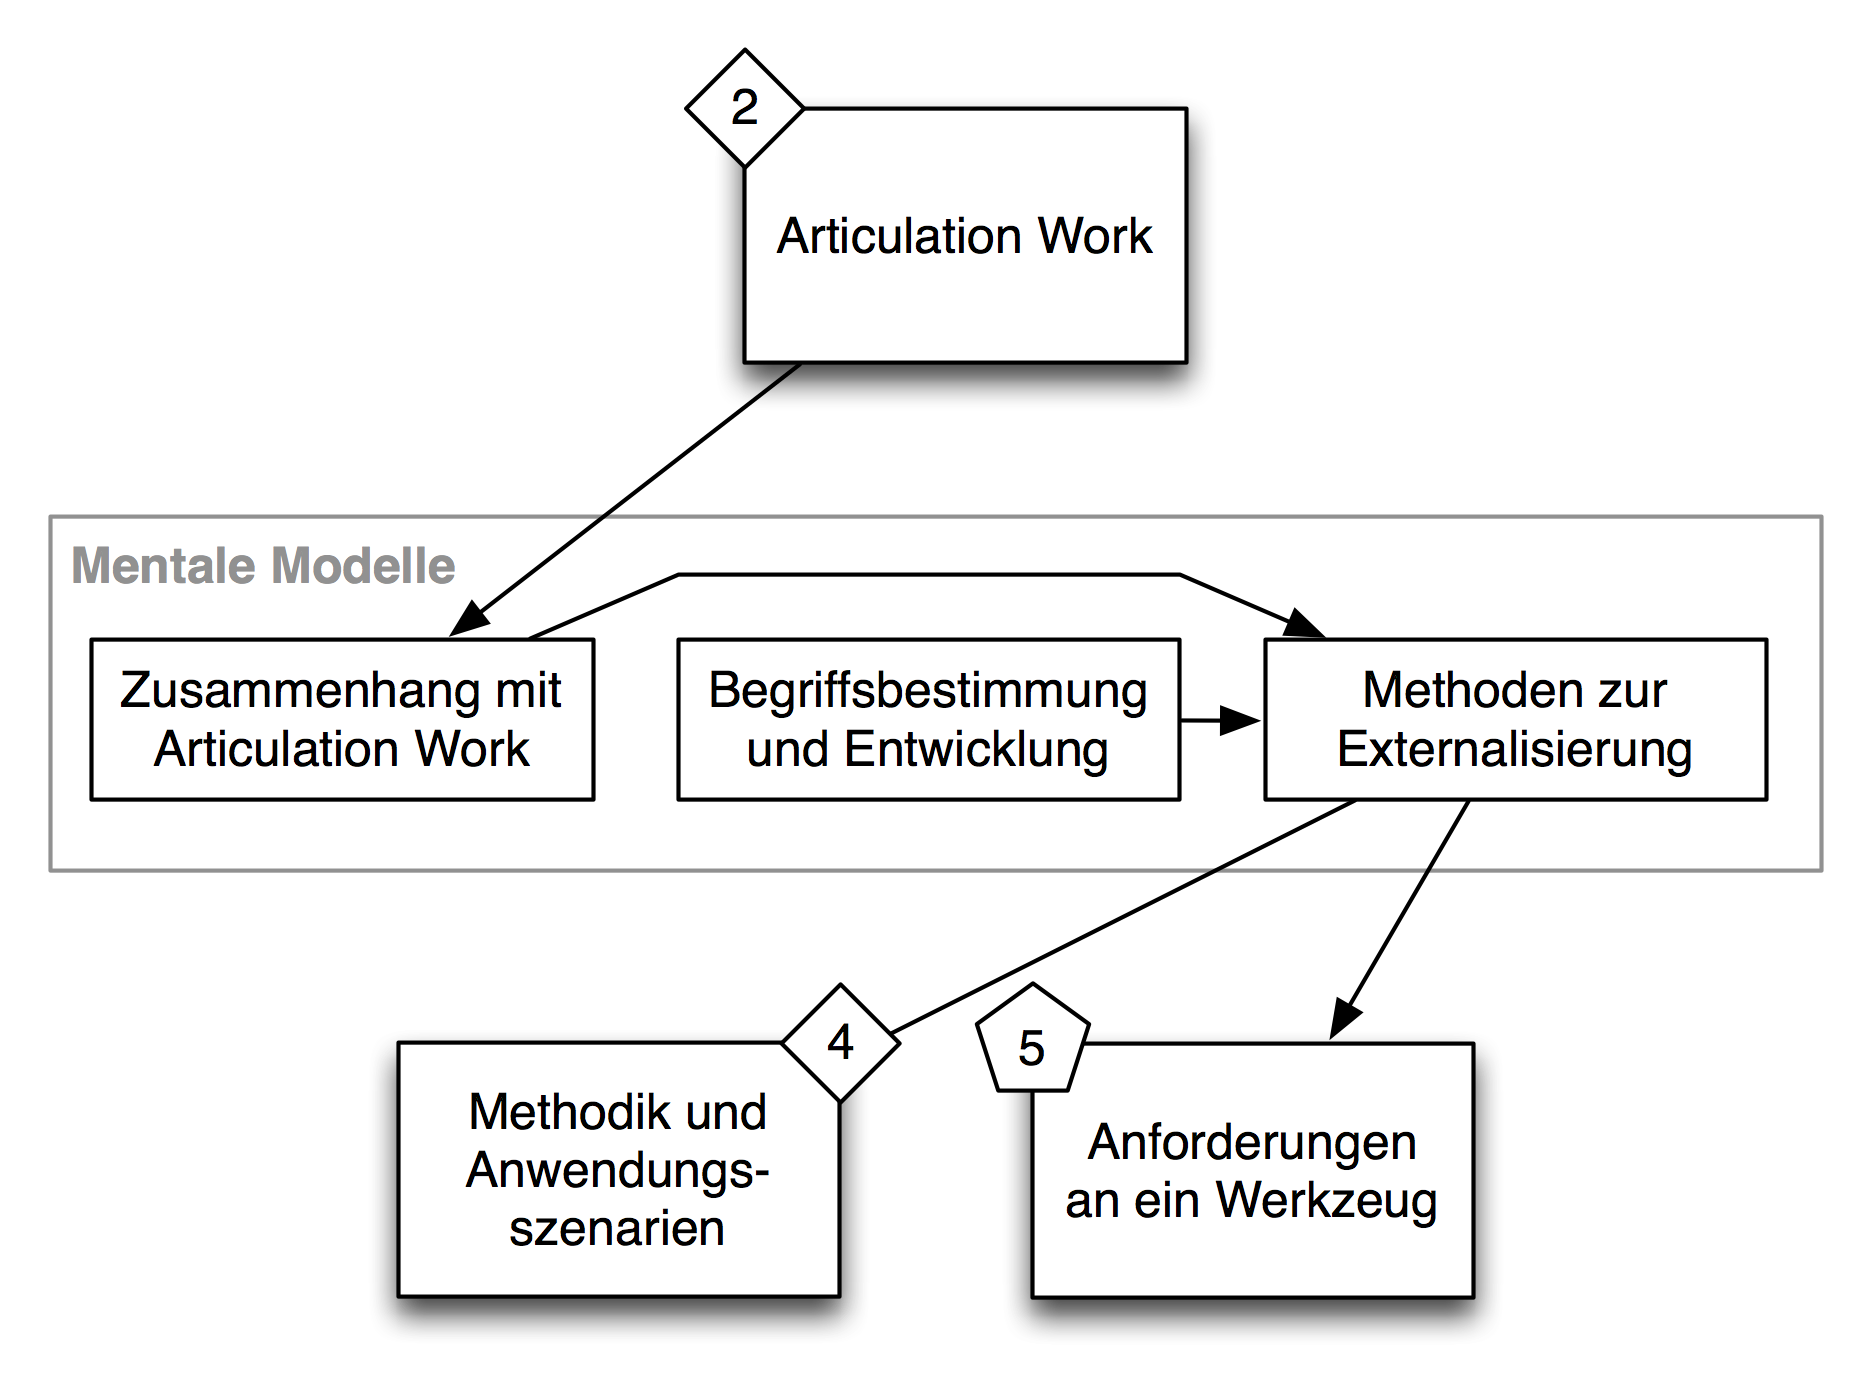
\includegraphics[scale=0.6]{img/Kontextgrafiken/k3.png}
	\caption{Kapitel „Mentale Modelle“ im Gesamtzusammenhang}
	\label{fig:img_Kontextgrafiken_k3}
\end{figure}

\section{Articulation Work und mentale Modelle} % (fold)
\label{sec:articulation_work_und_mentale_modelle}

Wie bereits im vorgehenden Kapitel beschrieben, werden in vorhandenen Arbeiten zu Articulation Work deren Auftreten, Kontext und Wirkung beschrieben, nicht aber jene Aspekte ihrer Durchführung, die die individuellen Aktivitäten betreffen. Der eigentliche Gegenstand der Abstimmung, die im Rahmen der Articulation Work erfolgen soll, wird ebenfalls nicht konkret festgelegt. Strauss spricht von \emph{„putting together tasks, task sequences, task clusters - even aligning larger units such as lines of work and subprojects - in the service of work flow“} \citep[][S. 2]{Strauss88}, und konkretisiert: \emph{„the specific questions about tasks of course include: what, where, when, how, for how long, how complex, how well defined are their boundaries, how attainable are they under current working conditions, how precisely are they defined in their operational details, and what is the expected level of performance. (Which of those are the most salient dimensions depends on the organizational work context under study, and we cannot emphasize too much that it is the researcher who must discover these saliences.)“} \citep[][S. 6]{Strauss85}. Strauss lässt also offen, was es exakt ist, dass abgestimmt werden muss bzw. verlagert diese Frage in den konkreten Einzelfall. 

Strauss spricht diese Auslassung in einer späteren Arbeit explizit an \citep[][S. 131]{Strauss93} und führt -- wie im letzten Kapitel bereits erwähnt -- das Konstrukt der „thought processes“ ein. Im Kontext der Abstimmung von Tätigkeiten kommt den „thought processes“ der Individuen insofern Bedeutung zu, als dass sie den sichtbaren individuellen Handlungen zugrunde liegen bzw. diese beeinflussen. „Articulation Work“ wirkt sich also auf die „thought processes“ der beteiligten Individuen aus. „Thought processes“ umfassen \emph{„images, imaginations, projections of scenes, [\ldots] flashes of insight, rehearsals of action, construction and reconstruction of scenarios,  the spurting up of metaphors or comparisons, the reworking and reevaluating of past scenes and one's actions within them, and so on and on“} \citep[][S. 130]{Strauss93} - also im Wesentlichen alle kognitiven Vorgänge, die unmittelbar oder mittelbar im Zusammenhang mit den sichtbaren Arbeitsaspekten, insbesondere den Tätigkeiten zur Zielerreichung und der wahrgenommenen Arbeitsumgebung, stehen. Strauss interessiert sich allerdings ausschließlich für die dynamischen Aspekte der Interaktion zwischen Individuen, nicht aber für die Ausgangspunkte und Ergebnisse der zugrunde liegenden „thought processes“ \citep[][S. 149]{Strauss93}.

% section articulation_work_und_mentale_modelle (end)

\section{Begriffsbestimmung} % (fold)
\label{sec:begriffsbestimmung}

% section begriffsbestimmung (end)

Das Konzept der „mentalen Modelle“ wird grundsätzlich verwendet, um zu erklären \emph{„wie Menschen die Welt verstehen -- genauer: wie sie ihr Wissen benutzen, um sich bestimmte Phänomene der Welt subjektiv plausibel zu machen“} \citep[][S. VII]{Seel91}. Mentale Modelle sind dabei Erklärungsmodelle der Welt, die von Menschen auf Basis von Alltagserfahrungen, bisherigem Wissen und darauf basierenden Schlussfolgerungen gebildet werden. Ein mentales Modell wird dann vom jeweiligen Individuum als Basis verwendet, um die Welt zu verstehen und ggf. Vorhersagen über deren Verhalten zu bilden. \citep[][S. VII]{Seel91}

Im Wesentlichen wurde das Forschungsfeld der mentalen Modelle durch zwei Arbeiten maßgeblich beeinflusst. \citet{Johnson-Laird81} sowie \citet{Kleer81} führen den Begriff als eigenständigen Forschungsgegenstand ein und legen damit die Grundlage für einen Großteil der nachfolgenden Arbeiten in dem Gebiet. Im Kontext dieser Arbeit wird auf das von \citet{Seel91} vorgeschlagene Verständnis von „mentalen Modellen“ zurückgegriffen. \citet{Seel91} versucht, die unterschiedlichen Richtungen der Forschung im Bereich der mentalen Modelle zusammenzuführen und daraus die Bedeutung von Mentalen Modellen für Lernvorgänge (unter die -- im breiten Verständnis von Seel -- auch die hier relevanten Abstimmungsvorgänge fallen) und Möglichkeiten zu deren Unterstützung abzuleiten. Die folgenden Ausführungen basieren deshalb auf den Ausführungen von \citeauthor{Seel91} und seiner Mitarbeiter (\citet{Ifenthaler06}, \citet{Pirnay-Dummer06} und \citet{Hanke06}).

Mentale Modelle sind nach \citet[][S. 7]{Ifenthaler06} \emph{„kognitive Konstruktionen, die abhängig von der jeweiligen Situation und vom semantischen Wissen einer Persone ad hoc konstruiert werden“}. Ein mentales Modell ist also kein permanentes kognitives Konstrukt, sondern wird auf Basis vorhandenen Wissens in bestimmten Situationen ad-hoc gebildet (siehe dazu auch Abschnitt \ref{sec:bildung_mentaler_modelle}). In engem Zusammenhang mit dem Begriff der mentalen Modelle ist jener der „Schemata“ zu nennen. „Schemata“ unterscheiden sich ihrer Definition nach nur in Detail von „mentalen Modellen“\footnote{Tatsächlich wird nach \citet{Ifenthaler06} der Begriff der „mentalen Modelle“ von manchen Autoren zugunsten von „Schemata“ als überflüssig bezeichnet, da zweitere die auftretenden kognitiven Phänomene ausreichend beschreiben würden.} Ein „Schema“ repräsentiert nach \citet[][S. 57]{Seel03a} \emph{„das aufgrund vielfältiger Einzelerfahrungen mit Objekten, Personen, Situationen und Handlungen erworbene verallgemeinerbare und abstrakte Wissen einer Person.“} Schemata werden benutzt um \emph{„Wissensstrukturen zu beschreiben, welche typische Zusammenhänge eines Realitätsbereiches repräsentieren.“} \citep[][S. 8]{Ifenthaler06}. Auf Basis dieser „Schemata“ treffen Individuen treffen Handlungsentscheidungen in bestimmten Situationen. „Schemata“ sind dabei als „Vorlagen“ zu sehen, die adäquate Handlungen für einen bestimmten Situationstypus vorgeben (im Sinne der erwähnten „Verallgemeinerbarkeit“) und Individuen damit zur raschen, unmittelbaren Handlung befähigt, ohne ausführliche Planungstätigkeiten durchführen zu müssen. In Abgrenzung dazu werden „mentale Modelle“ ad-hoc in Situationen gebildet, wo keine Schemata vorhanden sind oder vorhandene nicht angewandt werden können. 

\citet{Ifenthaler06} beschreibt den Zusammenhang zwischen Schemata und mentalen Modellen wie in Abbildung \ref{fig:img_MentaleModelle_iffenthaler_assimilation_akkommodation} dargestellt. Er bezieht sich dabei auf das „Äquilibrations“-Prinzip nach \citet{Piaget76}. Demnach entwickelt sich das Wissen eines Indiviuums durch die komplementären Prozesse „Assimilation“ und „Akkommodation.“

\begin{figure}[htbp]
	\centering		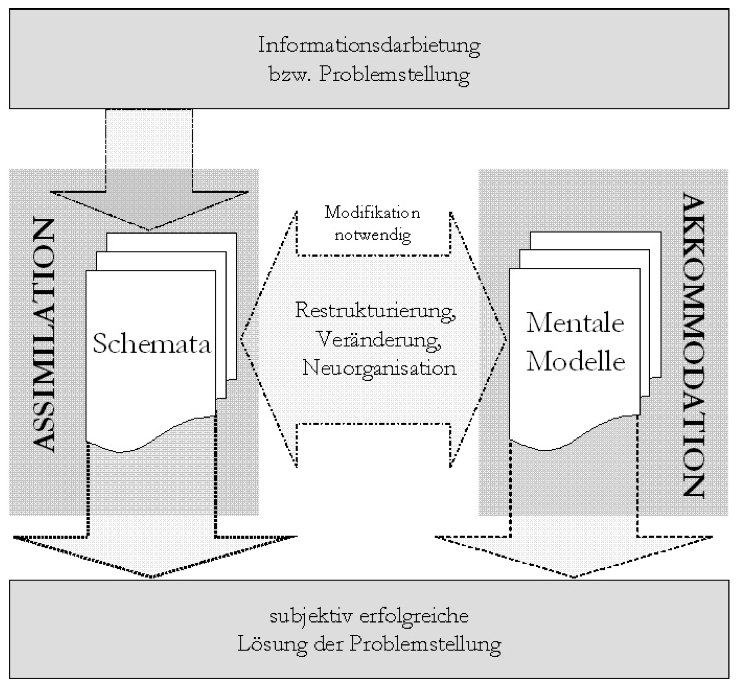
\includegraphics[height=3in]{img/MentaleModelle/iffenthaler_assimilation_akkommodation.png}
	\caption[Schemata und mentale Modelle]{Schemata und mentale Modelle (entnommen aus \citet[][S. 10]{Ifenthaler06})}
	\label{fig:img_MentaleModelle_iffenthaler_assimilation_akkommodation}
\end{figure}

Solange \wichtig eine wahrgenommene Situation auf existierende Schemata abgebildet werden kann und daraus unmittelbar Handlungen abgeleitet werden können, spricht man von „Assimilation“ der wahrgenommene Information. „Assimilation“ festigt bestehende Schemata, gestaltet diese ggf. in Details exakter aus oder um, stellt die grundlegenden Annahmen, die dem Schema zugrunde liegen, aber nicht in Frage. Kann die wahrgenommene Information nicht auf existierende Schemata abgebildet werden, kommt es zur „Akkommodation“, also der (ad-hoc) Bildung eines mentalen Modells und darauf aufbauend zur \emph{„Restrukturierung, Veränderung und Neuorganisation“} \citep{Ifenthaler06} der betreffenden Schemata. Schemata und mentale Modelle können damit auch als jene Strukturen interpretiert werden, die beim „Single-“ bzw. „Double-Loop-Learning“ nach \citet{Argyris78} zum Einsatz kommen. Im Kontext von „Articulation Work“ sind mentale Modelle in jenen Situation von Interesse, die als so „problematisch“ wahrgenommen werden, dass keine Fortführung der operativen Arbeit mehr möglich ist (auf individueller Ebene also evtl. existierende „Schemata“ nicht mehr zum Einsatz gebracht werden können). In diesen Situationen muss „explizite Articulation Work“ durchgeführt werden, um auf Basis eines mentalen Modells dieses selbst zu verändern, auszugestalten und soweit mit der Umwelt abzustimmen, das eine Wiederaufnahme der operativen Arbeit (bzw. die Bildung von adäquaten Schemata) möglich wird. Um auf die Durchführung von „expliziter Articulation Work“ unter Bezugnahme auf die mentalen Modelle der Individuen näher eingehen zu können, werden im nächsten Abschnitt die Bildung und Veränderung mentaler Modelle näher betrachtet.

\section{Bildung und Veränderung mentaler Modelle} % (fold)
\label{sec:bildung_mentaler_modelle}

Nach \citet{Seel91} umfasst die Bildung mentaler Modelle zwei Komponenten: Eine \emph{deklarative Komponente}, in der bereichs- bzw. domänen-spezifisches Wissen in der Form von hier nicht näher spezifizierten, strukturierten Wissensbasen abgelegt wird und eine \emph{operative Komponente}, in der auf Grundlage dieser Wissensbasen Schlüsse gezogen und neues Wissen abgeleitet wird, die über das ursprüngliche domänenspezifische Wissen hinausgeht. 

Das in den Wissensbasen repräsentierte Wissen kann auf Alltagserfahrung basieren oder durch Vermittlung oder Instruktion begründet werden. Im ersteren Fall ist das Wissen dann als konkret und handlungsbezogen anzusehen, im zweiten Fall ist das Wissen eher auf abstrakter, formaler Ebene anzusiedeln. Analog dazu kann auch in der operativen Komponente die Schlussfolgerung entweder induktiv auf Basis eines „intuitionsbegründeten“ Regelsystems gezogen werden oder durch Deduktion mittels einem formal begründbaren Regelsystem gebildet werden \citep{Seel91}. 

Die Modifikation und Erweiterung der eigenen Wissensbasen und die (Weiter-) Entwicklung der kognitiven Fähigkeiten, die für die Ableitung von Schlussfolgerungen notwendig sind, bezeichnet \citet{Seel91} als „Lernen“. Lernen ist \emph{"mit der Verarbeitung individueller Erfahrungen mit sowie vermittelter Information über die Welt, ihre Struktur und Evidenz verbunden und kann als ein Prozess permanenter konzeptueller Veränderungen verstanden werden."} \citep[][S. 23]{Seel91}. Lernen setzt damit die Fähigkeit und Bereitschaft voraus, \emph{"vermittelte Weltauffassungen zu verstehen, zu akzeptieren und sodann den eigenen gedanklichen Konstruktionen zugrunde zu legen"} \citep[][S. 23]{Seel91}. Im Wesentlichen entspricht dies einer Verallgemeinerung jener Vorgänge, die im Rahmen von nicht rein koordinierender sondern abstimmender und vor allem planender „Articulation Work“ durchgeführt werden.

In Zusammenhang mit diesem Verständnis von „Lernen“ sind verschiedene Arten von mentalen Modellen zu unterscheiden. \citet{Seel91} differenziert zwischen „Novizenmodellen“ und „Expertenmodellen“ (diese Unterscheidung trifft implizit auch \citet{Norman83a} im Kontext der Verwendung mentaler Modelle in der \gls{HCI}). Ein „Novizenmodell“ ist ein Alltagsmodell, dass ad-hoc in einer Problemsituation gebildet wird und dem Individuum, das es gebildet hat, in der aktuellen Situation plausibel erscheint (auch wenn es objektiv falsch ist). Es reicht aus, um adäquate Reaktionen auf die gegebene Situation abzuleiten, ohne das notwendigerweise eine Begründung der Handlungen möglich wäre oder diese nicht mit dem tatsächlichen Grund der Problembewältigung übereinstimmen\footnote{\emph{„[\ldots] most people’s understanding of the devices they interact with is surprisingly meager, imprecisely specified, and full of inconsistencies, gaps and idiosyncratic quirks.“}\citep[][S. 8]{Norman83a}}. Je öfter die Anwendung eines „Novizenmodells“ zum Erfolg führt, umso stabiler wird es zur Grundlage des Handelns des Individuums in der jeweiligen Situation. 

„Expertenmodelle“ (oder „wissenschaftliche Modelle“) sind hingegen inhaltlich vollständiger und bilden die Ursache-Wirkungs-Zusammenhänge der beobachtbaren Realität ab (sind also „objektiv korrekt“). Sie sind im allgemeinen differenzierter und bedienen sich einer adäquateren mentalen Codierung -- d.h. Begriffssystem -- als „Novizensysteme“ (die sich i.A. vertrauter Begriffssysteme bedienen, auch wenn diese einer anderen Domäne entstammen oder objektiv inkorrekt sind). Auch die Kompetenz des Individuums im Umgang mit dem mentalen Modell ist in diesem Fall höher. Der Übergang von einem „Novizenmodell“ zu einem „Expertenmodell“ erfolgt dabei durch „Lernen“ im oben genannten Sinn. \citep{Ifenthaler06}

„Expertenmodelle“ müssen aber nicht immer den erwünschten Endzustand eines Lernprozesses darstellen. Durch die gesteigerte Komplexität des Modells wird dessen ad-hoc-Anwendung schwieriger, die Nützlichkeit des Modells ist deshalb eingeschränkt \citep[vgl. ][S. 20]{Ifenthaler06}. Hier zeigt sich eine Analogie mit dem Bereich „Articulation Work“, wo es -- wie im letzten Kapitel beschrieben -- ebenfalls nicht als erforderlich angesehen wird, dass jedes beteiligte Individuum eine detaillierte Gesamtsicht auf den Arbeitsablauf hat. Vielmehr ist es ausreichend, die jeweils relevanten Schnittstellen zu abzustimmen und einen groben Überblick über den Gesamtzusammenhang zu haben. 

\citet{Ifenthaler06} erweitert deshalb die binäre Klassifikation durch „Erklärungsmodelle“, die er konzeptionell zwischen „Novizen-“ und „Expertenmodellen“ ansiedelt. Ein „Erklärungsmodell“ \emph{„beinhaltet alle notwendigen Informationen, um ein Problem bezüglich des Sachverhaltes und der Anforderungssituation richtig zu lösen. Einem Erklärungsmodell wird dabei ein hoher Grad an Nützlichkeit beigemessen, was in Bezug auf die kognitive Leistung zu einer ergonomischen Problemlösung führt. Je nach Komplexität des Sachverhaltes und der damit verbundenen Anforderungssituation kann ein Erklärungsmodell einem Novizenmodell oder einem Expertenmodell sehr ähnlich sein“} \citep[][S. 21]{Ifenthaler06}. „Erklärungsmodelle“ sind also je nach Art der zugrunde liegenden Problemstellung unterschiedlich aufgebaut. Ziel eines „Erklärungsmodells“ ist es immer, bestmöglich zur Problemlösung beizutragen, diese also für das Individuum im Kontext der jeweiligen Problemstellung möglichst einfach zu gestalten. Ein „Erklärungsmodell“ gewinnt dabei durch „Lernen“ an Reifegrad, es nähert sich einem „Expertenmodell“ immer weiter an.

Im \wichtig Kontext von „Articulation Work“ ist der Begriff des „Erklärungsmodells“ ein hilfreiches Konstrukt. Je nach Reifegrad des betreffenden mentalen Modells wird eine bestimmte Arbeitssituation als mehr oder weniger komplex wahrgenommen. Je komplexer eine Arbeitssituation wahrgenommen wird, desto größer ist der Bedarf nach expliziter „Articulation Work“, also der expliziten Beschäftigung mit dem Arbeitsprozess, dessen Reflexion und der Abstimmung der eigenen Wahrnehmung mit anderen beteiligten Individuen. Diese Beschäftigung mit dem Arbeitsprozess, also jene Tätigkeiten, die im Rahmen der „Articulation Work“ durchgeführt werden, entsprechen -- wie oben bereits beschrieben -- dem hier beschriebenen „Lernen“, wobei in kooperativen Arbeitssituation die Quellen „vermittelter Information“ vorrangig die anderen beteiligten Individuen oder organisationale Artefakte sind, die den Arbeitsablauf beschreiben. 

Die Veränderung mentaler Modelle weist zwei grundlegende Schwierigkeiten auf. Bei bereits als nicht adäquat erkannten mentalen Modellen (wie sie bei „Articulation Work“, die in „non-routine work“ bzw. „problematic work“ ausgeführt wird, auftreten), besteht grundsätzlich die Bereitschaft zur Veränderung (im Sinne einer „Akkommodation“ des mentalen Modells an die als verändert wahrgenommene Umweltbedingungen), die Herausforderung besteht aber darin, die notwendigen Informationen vermittelt zu bekommen, also an diese zu gelangen und adäquat dargeboten zu bekommen. Eine weitere Schwierigkeit ergibt sich in Situationen, in denen nicht alle involvierten Individuen die Situation als „problematisch“ wahrnehmen und deshalb keine grundlegende Bereitschaft zeigen, ihre der Arbeit zugrunde liegenden Annahmen (also ihre mentalen Modelle) zu verändern (\citet{Ifenthaler06} spricht von „hoher Veränderungsresistenz“). Dies tritt vor allem im Situationen auf, in denen „Articulation Work“ nicht aus einer allgemein wahrgenommen Problemsituation heraus durchgeführt wird, sondern entweder mit rein planendem Charakter angestoßen wird oder nur für einzelnen beteiligte Individuen so stark „problematisch“ ist, dass eine explizite Beschäftigung mehrerer oder aller am Arbeitsablauf beteiligten notwendig ist. 

Aus der Theorie der mentalen Modelle heraus begründet müssen also drei Rahmenbedingungen gegeben sein, um „explizite Articulation Work“ durchführen zu können:
\begin{enumerate}
	\item Die Beteiligten müssen bereit sein, ihre mentalen Modelle abzustimmen und das individuelle Verständnis der Schnittstellen abzugleichen.
	\item Die von den beteiligten Individuen benötigte Information über den Arbeitsablauf muss von den anderen Beteiligten zur Verfügung gestellt werden können oder in der Form organisationaler Artefakte vorliegen.
	\item Die benötigte Information muss in adäquater Form dargeboten werden, um  die individuellen mentalen Modelle mit diesen in Einklang zu bringen.
\end{enumerate}

Anforderung 1 ist eine Frage des sozialen Verhaltens der beteiligten Personen bzw. der Organisationskultur und kann ggf. durch organisationale Maßnahmen (z.B. durch die Förderung von „Communities of Practice“ \citep{Wenger99}) unterstützt werden. Anforderung 2 kann trivial zu erfüllen sein, wenn der Kontext des Arbeitsablaufs (d.h. das Umfeld, in dem die Arbeit durchgeführt wird, u.a. inkl. aller beteiligten Individuen) bekannt ist. In komplexen, neuartigen oder unbekannten Arbeitssituationen muss auch die Erfüllung dieser Anforderung unterstützt werden. Ansatzpunkte dafür liefert im Bereich von „Articulation Work“ etwa \citet{Grinter96} (siehe Abschnitt \ref{sub:supporting_articulation_work_using_software_configuration_management_systems}) oder \citet{Fuchs01} (siehe Abschnitt \ref{sub:teamspace}), umfassend mit dieser Thematik beschäftigt sich der Forschungsbereich der „Organisational Memories“ (zur technischen Unterstützung siehe etwa \citep{Abecker98} oder \citep{Diefenbruch02}\footnote{eine detaillierte Darstellung des Forschungsgebiets ist in \citep{Maier08} zu finden}).

Anforderung 3 wird in der Forschung zum Thema „Articulation Work“ von \citet{Sarini02} im Kontext des „alignment of meanings“ angesprochen, bei dem eine automationsgestützte Abbildung unterschiedlicher Domänenvokabulare die grundsätzliche Verständigung bzw. die Vermeidung von Missverständnissen vermeiden soll. Diese Maßnahme ermöglicht allerdings erst die Abstimmung mentaler Modelle, unterstützt diese aber noch nicht unmittelbar. Im Sinne der adäquaten Form der Darbietung argumentieren auch \citet{Divitini00}, \citep{Jorgensen04} und vor allem \citet{Herrmann02} mit der Forderung von flexiblen bzw. an die Bedürfnisse der Benutzer anpassbaren Modellierungsprachen bei der Verwendung von externalisierten Modellen als Unterstützung der Durchführung von „Articulation Work“ (siehe dazu die Abschnitte \ref{sub:supporting_different_dimensions_of_adaptability}, \ref{sub:interactive_process_models} und \ref{sub:modelling_cooperative_work}).

Hinsichtlich \wichtig Anforderung 3 argumentiert \citet{Seel91} im Bereich der mentalen Modelle für die Nützlichkeit externalisierter Repräsentationen zur Verbesserung von mentalen Modellen. Er vertritt die Auffassung, dass „die Externalisierung die Konstruktion eines mentalen Modells 'vervollkommnet'“, was er darauf zurückführt, dass „erst aus der Zielsetzung heraus, sich einem anderen mitzuteilen, die Präzision einer gedanklichen Konstruktion resultiert, die für die Erklärung einer Weltergebenheit erforderlich ist“ \citep[][S. 155]{Seel91}. Die Bildung von Externalisierungen mentaler Modelle verbessert also einerseits das individuelle mentale Modell, indem sie Lücken und Inkonsistenzen bewusst macht, und ermöglicht andererseits die Kommunikation mit anderen Individuen und ist damit die Grundlage der Vermittlung von Information und damit des „Lernens“ und „Articulation Work“ im hier beschriebenen Sinn. \citet{Seel91} lässt jedoch offen, in welcher Form die Repräsentation erfolgt, um die Vermittelbarkeit bestmöglich sicherzustellen\footnote{\emph{„Internalisierung von Erkenntnismitteln setzen Zeichensysteme (auditiver, visueller oder anderer Natur) für die Verschlüsselung der semantischen Gebilde voraus“}\citep[][S. 155]{Seel91}}. \citet{Ifenthaler06}, \citet{Hanke06} und \citet{Pirnay-Dummer06} weisen an dieser Stelle jedoch auf qualitative Unterschiede der Eignung unterschiedlicher externer Repräsentationsformen mentaler Modelle zur Externalisierung und Vermittlung derselben hin. Auf diese unterschiedlichen Formen und deren Eignung wird im nächsten Abschnitt eingegangen. 

Grundsätzlich konnte jedoch hier gezeigt werden, dass „Articulation Work“ die mentalen Modelle der beteiligten Individuen verändert bzw. auf diesen aufbaut. In weiterer Folge wurde deutlich, dass zur expliziten Durchführung von „Articulation Work“ auch aus der Theorie der mentalen Modelle heraus die Verwendung von externalisierten Modellen (wie bereits von \citet{Divitini00}, \citet{Herrmann02} und \citet{Jorgensen04} ohne den Hintergrund der mentalen Modelle vorgeschlagen) sinnvoll ist.

Diese Forderung nach einer Externalisierung mentaler Modelle, um deren Abstimmung zu unterstützten wird auch durch die Ausführungen von \citet{Senge90} und \citet{Kim93} gestützt, die mentale Modelle\footnote{in einem etwas breiteren Verständnis, welches im Wesentlichen auch Schemata umfasst: \emph{„[mental models are] deeply ingrained assumptions, generalizations, or even pictures and images that influence how we understand the world and how we take action.“}\citet{Senge90}} als ein wichtiges Konzept im Kontext des organisationalen Lernens identifizieren. Mentale Modelle bilden dort die Grundlage für Handlungen von Individuen in Organisationen und müssen geteilt werden, um der Organisation selbst eine Weiterentwicklung (einen „organisationalen Lernschritt“) zu ermöglichen.
% section bildung_mentaler_modelle (end)

\section{Externalisierung mentaler Modelle} % (fold)
\label{sec:externalisierung_mentaler_modelle}

Die Externalisierung von „mentalen Modellen“ ist immer ein zweistufiger Prozess (siehe Abbildung \ref{fig:img_MentaleModelle_iffenthaler_externalisierung}), in dem jeweils eine Transformation des Kodierungssystems stattfindet. Die wahrgenommene Realität (das „Weltwissen“) wird (ad-hoc) in ein mentales Modell abgebildet werden. Soll dieses externalisiert werden, ist dazu ein weiterer Übersetzungs- bzw. Abbildungsschritt notwendig. Gleichzeitig führt nach \citet{Stachowiak73} jede Modellbildung neben der „Abbildung“ auch zur „Verkürzung“, d.h. dass das Modell nicht die gesamte Information des Originals enthält, sondern nur jene Aspekte, die dem Ersteller relevant erscheinen\footnote{\emph{„Modelle erfassen im allgemeinen nicht alle Attribute des durch sie repräsentierten Originals, sondern nur solche, die den jeweiligen Modellerschaffern und/ oder Modellbenutzern relevant scheinen.“}\citep{Stachowiak73}}. In diesem Sinne können sie nur in einem bestimmten (zeitlichen, personellen und operationalen) Kontext für das Original stehen („pragmatisches Merkmal“ -- jedes Modells ist für einen bestimmten Zweck konstruiert\footnote{\emph{„Modelle sind ihren Originalen nicht per se eindeutig zugeordnet. Sie erfüllen ihre Ersetzungsfunktion: für bestimmte — erkennende und/ oder handelnde, modellbenutzende — Subjekte; innerhalb bestimmter Zeitintervalle und unter Einschränkung auf bestimmte gedankliche oder tatsächliche Operationen.“}\citep{Stachowiak73}}).

\begin{figure}[htbp]
	\centering
		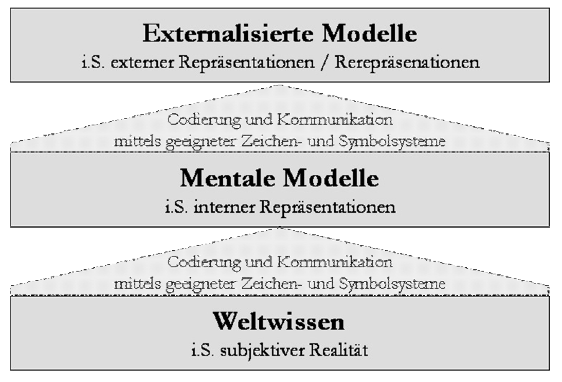
\includegraphics[width=8cm]{img/MentaleModelle/iffenthaler_externalisierung.png}
	\caption[Externalisierung mentaler Modelle]{Externalisierung mentaler Modelle (entnommen aus \citep{Ifenthaler06})}
	\label{fig:img_MentaleModelle_iffenthaler_externalisierung}
\end{figure}

Herausfordernd ist im Kontext von „Articulation Work“ das Abbildungsmerkmal, also die notwendige Übersetzungsleistung bei der Externalisierung eines mentalen Modells. Externalisierung umfasst nach \citet{Hanke06} immer die „Repräsentation“ als auch die „Kommunikation“ eines mentalen Modells. Die Relevanz dieser beiden Aspekte verschiebt sich je nach Kontext bzw. Zielsetzung der Externalisierung. Dient diese eher der individuellen Verständnisbildung, steht die „Repräsentation“ im Vordergrund (diesen Zweck erfüllt nach \citep{Seel91} auch bereits das mentale Modell selbst, die Externalisierung hat schärfenden Charakter). Die externalisierte Repräsentation soll nach \citet[][S. 187]{Seel91} in Bezug auf das repräsentierte mentale Modell
\begin{itemize}
	\item vollständig 
	\item konzise
	\item kohärent und konkret
	\item bedeutungshaltig und korrekt
\end{itemize}
sein. Das \wichtig Kodierungssystem muss hier also so gewählt werden, dass eine möglichst unmittelbare Abbildung der mentalen Modelle auf die externalisierte Repräsentation (und vice versa) möglich ist. 

In Situationen, in denen mentale Modelle zusätzlich auch anderen Individuen vermittelt werden sollen, steht „Kommunikation“ im Vordergrund. Die „Kommunizierbarkeit“ eines mentalen Modells hat Auswirkungen auf die wählbaren Kodierungssysteme zur Externalisierung. Das gewählte Kodierungssystem muss allen beteiligten Individuen verständlich sein, während dieses Kriterium bei der individuellen Verständnisbildung irrelevant ist \citep{Hanke06}. Im Rahmen von „Articulation Work“ steht im Allgemeinen die „Kommunikation“ bei der Externalisierung im Vordergrund, wobei diese ohne eine adäquate „Repräsentation“ nicht möglich ist. \label{anforderungen_seel} Ziel muss es also sein, Kodierungssysteme zur Verfügung zu stellen, die 
\begin{itemize}
	\item allen beteiligten Individuen verständlich sind, und
	\item eine möglichst unmittelbare Abbildbarkeit der mentalen Modelle auf die externalisierte Repräsentation ermöglicht.
\end{itemize}

Kodierungssysteme können \emph{„auditiver, visueller oder anderer Natur“} \citep[][S. 155]{Seel91} sein. Das gebräuchlichste Kodierungssystem ist die natürliche Sprache. Diese ist im Sinne der ersten Anforderung oft eine gute Wahl, bietet aber aufgrund ihrer Generizität nur wenig Möglichkeiten, sowohl den Repräsentations- als auch den Kommunikationsprozess bei der Externalisierung explizit zu unterstützen. \citet{Ifenthaler06} stellt mehrere Methoden vor, die sich spezifisch zum Zwecke der Externalisierung mentaler Modelle eignen und zu qualitativ höherwertigen Externalisierungsergebnisse führen sollen. Dies sind im Einzelnen:
\begin{itemize}
	\item Methode des lauten Denkens
	\item Strukturlegetechniken
	\item Concept Mapping
\end{itemize}

Auch \citep{Huss03} erwähnt diese Ansätze im Zusammenhang mit der Externalisierung „mentaler Repräsentationen“. In der Folge werden die genannten Ansätze detaillierter betrachtet. Dabei kommt folgender Raster zum Einsatz:
\begin{description}
	\item[Konzept] beschreibt die grundlegenden Konzepte des Ansatzes und die darauf aufbauende Zielvorstellung
	\item[Vorgehen] beschreibt, wie die Zielerreichung methodisch sichergestellt werden soll. 
	\item[Unterstützung] beschreibt, welche (technischen) Unterstützungsmaßnahmen vorgeschlagen werden.
	\item[Bewertung] fasst die Eigenschaften der Methode zusammen und beurteilt sie hinsichtlich ihrer Eignung für „Articulation Work“
\end{description}

\subsection{Methode des lauten Denkens} % (fold)
\label{sub:methode_des_lauten_denkens}

Die „Methode des lauten Denkens“ \citep{Van-Someren94} beschreibt ein Vorgehen, bei dem Individuen während ihrer operativen Tätigkeit ihre Gedanken und die Motive für ihr Handeln verbalisieren. 

\subsubsection{Konzept}

Die Grundidee des „Methode des lauten Denken“ basiert darauf, alle Gedanken, die im eine Tätigkeit begleiten, laut auszusprechen ohne sich auf diese Verbalisierung explizit zu konzentrieren (und etwa über Formulierungen nachzudenken oder Interpretationen durchzuführen). Es werden keine Fragen gestellt, das externalisierende Individuum wird ggf. lediglich daran erinnert, seine Gedanken auszusprechen. Nach \citet{Van-Someren94} hat diese Form der Externalisierung keinen negativen Einfluss auf die Durchführung der eigentlichen Tätigkeit.

Die „Methode des lauten Denkens“ wird immer mit dem Ziel durchgeführt, die kognitiven Prozesse in einer bestimmen Situation offenzulegen. Dazu muss eine Problemstellung ausgewählt werden, die diese Situation auslöst und möglichst keine oder geringe Nebeneffekte aufweist. Zu diesen Nebeneffekten gehört etwa die kognitive Überforderung des Individuums, wenn die Aufgabe als zu schwierig wahrgenommen wird. Gleichzeitig führt eine zu einfache Aufgabe zu eine routinisierten Abarbeitung, deren kognitiven Prozesse zumeist implizit und schwer zu externalisieren sind (vgl. „Operations“ in der „Activity Theory“ \citep{Leontev78}). Der wahrgenommene Schwierigkeitsgrad der Aufgabe steht in direktem Bezug mit der Expertise des Individuums (als unabhängige Variable), die damit bei der Auswahl der Problemstellung berücksichtigt werden muss.

Die „Methode des lauten Denkens“ wird oft mit Retrospektion kombiniert. Retrospektion ist die angeleitete Reflexion über eine Tätigkeit im Nachhinein (also nach Abschluss der Tätigkeit). Im Falle der Kombination mit der „Methode des lauten Denkens“ wird diese Reflexion mit Protokollen der verbalisierten Gedanken durchgeführt, was Unklarheiten in diesen Protokollen beseitigt und eine tiefergehende Reflexion ermöglichen kann. 

Die Ergebnisse der „Methode des lauten Denkens“ werden auf Basis von Audio- oder Video-Aufnahmen möglichst exakt transkribiert. Die Auswertung der Protokolle erfolgt im Normalfall nicht durch das Individuum selbst sondern wird interpretativ durch Dritte durchgeführt. Von \citet{Van-Someren94} wird dazu unter anderem vorgeschlagen, eine Aufgaben-Analyse durchzuführen, deren Ergebnis im Allgemeinen ein (diagrammatisches) Modell der Aufgaben und Tätigkeiten des Individuum zur Zielerreichung ist.

\subsubsection{Vorgehen}

\citet{Van-Someren94} beschreiben einen prototypischen Ablauf der „Methode des lauten Denkens“, der hier angegeben wird. Die Durchführung der Methode sollte in einer möglichst ungestörten, ruhigen Umgebung erfolgen. Das Individuum wird instruiert, bei der Problemlösung laut mitzusprechen und alles zu sagen, was ihm durch den Kopf geht (für konkrete Formulierungsvorschläge der Fragestellungen siehe \citep[][S. 43]{Van-Someren94}). Bevor die eigentliche Problemstellung bekannt gegeben wird, kann bei in der Methode ungeübten Individuen eine „Aufwärmphase“ durchgeführt werden, in der etwa anhand der Lösung einer einfachen Schlussrechnung das Verbalisierung der Überlegungen zu deren Lösung geübt werden kann.

Während der Durchführung der Methode beschränkt sich der Untersuchungsleiter darauf, das Individuum an das Aussprechen seiner Gedanken zu erinnern, sobald dieses zu sprechen aufhört. Der gesamte Verlauf der Aufgabenbearbeitung wird mittels Audio- oder Video-Ausrüstung aufgezeichnet.

Nach Abschluss der Methode wird die gesamt Aufzeichnung transkribiert. Bei der Transkription muss auf höchste Exaktheit geachtet werden, auch Sprechpausen oder nichtverbale Geräusche des Individuums sind relevant. Liegt eine Videoaufzeichnung vor, so wird das Transkript um die beobachteten Tätigkeiten des Individuums ergänzt. Das fertige Transkript kann dem Individuum im Sinne der Retrospektion zur Kommentierung vorgelegt werden, bei der Ergänzungen oder Erklärungen angebracht werden können (aber als solche gekennzeichnet werden müssen).

Zur Auswertung der Ergebnisse der „Methode des lauten Denkens“ werden unterschiedliche Methoden herangezogen, im im Detail in \citep{Van-Someren94} beschrieben sind. Da hier lediglich die Externalisierung selbst von Interesse ist, wird auf diese Methode an dieser Stelle nicht näher eingegangen.

\subsubsection{Unterstützung}

Eine technische Unterstützung der „Methode des lauten Denkens“ ist von den Entwicklern der Methode \citep{Van-Someren94} grundsätzlich nicht vorgesehen. Lediglich zur Dokumentation der artikulierten Information wird eine Aufzeichnung mittels Video- oder Audio-Ausrüstung empfohlen. Diese Dokumentation ist notwendig, um eine möglichst vollständige Auswertung der Information zu gewährleisten und eine Abbildung auf eine strukturierte Externalisierung des zugrunde liegenden mentalen Modells zu ermöglichen. 

\citet{Senge90} schlägt zur verbalen Externalisierung von mentalen Modellen einen Ansatz vor, der der „Methode des lauten Denkens“ nahe kommt, die Gedanken des Individuums aber verschriftlicht. Bei Einsatz der „left-hand column“\footnote{Eine detaillierte Beschreibung der Methode ist in \citep{Senge94} erschienen} wird ein Blatt Papier in zwei Spalten geteilt, wobei in der rechten Spalte eine Transkription der Handlungen bzw. der Konversation eines Individuums eingetragen wird. In der linken Spalte werden die Gedanken und handlungsmotivierenden Überlegungen eingetragen und den sichtbaren Handlungen in der rechten Spalte zugeordnet. Ein Nachteil dieser Methode ist, dass er -- auch wenn er technisch unterstützt werden würde -- nur im Nachhinein durchgeführt werden kann, um den eigentlichen Arbeitsablauf nicht zu unterbrechen.

\subsubsection{Bewertung}

Die „Methode des lauten Denkens“ \citep{Van-Someren94} ist die einzige der vorgeschlagenen Methoden zur Externalisierung mentaler Modelle, welche nicht auf eine graphische Repräsentationsform zurückgreift. Die externalisierende Person muss während der Aufgabenbearbeitung unmittelbar ihre kognitiven Prozesse und Denkmuster verbalisieren. Dies ist für viele Menschen ungewohnt und führt oft zu unvollständigen Repräsentationen. Detailliertes Nachfragen ist hier deshalb notwendig. Die gewonnen Daten (etwa aus Audio- oder Videomitschnitten des Versuchsszenarios) werden strukturiert ausgewertet, kategorisiert und interpretiert. Hier liegt auch die Schwierigkeit des Verfahrens -- in der Interpretation ist eine eindeutige Zuordnung zu bestimmten kognitiven Prozessen oft nicht möglich, die Repräsentation des mentalen Modells bleibt unvollständig oder ist inkonsistent. \citep[][S. 28]{Ifenthaler06}

In einer informellen Variante ist die „Methode des lauten Denkens“ jedoch vor allem für den Einsatz in nicht komplexen Fällen von „Articulation Work“ geeignet (also etwa bei kleineren Änderung im Arbeitskontext, die die Anpassung einzelner Tätigkeiten aber nicht die Adaption des gesamten Arbeitsablaufs benötigen). Dabei kann auf eine Aufzeichnung ggf. verzichtet werden, da die Durchführung der unmittelbaren Kommunikation dient und deren Ergebnisse nicht weiter interpretiert oder anderweitig verwendet werden müssen.

% subsection methode_des_lauten_denkens (end)

\subsection{Strukturlegetechniken} % (fold)
\label{sub:strukturlegetechniken}

Strukturlegetechniken sind Methoden, in denen gelegte Strukturen zur Repräsentation von „Wissen“ eingesetzt werden. Die gelegten Strukturen (die im Wesentlichen aus Knoten und Kanten unterschiedlicher Bedeutung bestehen) bilden dabei die Zusammenhänge einzelner Konstrukte ab, wie sie die legende Person wahrnimmt. Der Prozess des Legens ist eine \emph{„Rekonstruktion subjektiver Theorien“} \citep{Dann92} und stellt eine \emph{„[\ldots] verstehende Beschreibung von Handlungen nicht aus der Perspektive eines außenstehenden Beobachters, sondern aus Sicht der handelnden Person, des Akteurs selber“} \citep[][S. 2]{Dann92} dar.

\subsubsection{Konzept}

Das Konzept der Strukturlegetechniken entstammt im Wesentlichen einem Forschungsprogramm zur Entwicklung von Ansätzen zur „rekonstruktiven Erhebung subjektiver Theorien“ \citep{Dann92}. „Subjektive Theorien“ sind dabei im Wesentlichen den mentalen Modellen und Schemata gleichzusetzen\footnote{\emph{„Subjektive Theorien [\ldots] sind nicht nur unmittelbar handlungserklärend, -rechtfertigend oder –leitend; d.h. sie beziehen sich über die unmittelbare Erklärung/Rechtfertigung etc. eigener Handlungen hinaus auf z.B. ganze Handlungskategorien [\ldots]“} \citep[][S. 34]{Scheele88}} \citep[][zitiert nach \citep{Huss03}]{Kluwe90}. Strukturlegetechniken sind nicht als reine Erhebungsmethoden zu sehen, sondern beeinflussen durch den Lege-Vorgang selbst die zu externalisierenden mentalen Modelle und bilden damit die Grundlage für eine mögliche Veränderung des Agierens im Arbeitskontext \citep[][S. 6]{Dann92}.
Die Grundidee von Strukturlegetechniken ist die freie Anordnung und Assoziation von Begriffen. Je nach Variante kann dies individuell oder in Gruppen, mit oder ohne Moderator bzw. Untersuchungsleiter geschehen. Der Prozess ist dann abgeschlossen, wenn die Beteiligten die Repräsentation als eine adäquate Abbildung ihrer Denkmodelle sehen. Vor allem in kooperativen Sitzungen ist dies mit Aushandlungs- und Abstimmungsprozessen während der Repräsentation verbunden, was Strukturlegetechniken in der Durchführung potentiell aufwändig macht.

Strukturlegetechniken sind hinsichtlich der Art und dem Umfang der vorgegebenen Konstrukte nicht einheitlich aufgebaut. Es existieren Ansätze, in denen sämtliche Strukturelemente (also Konzepte und Arten von Beziehungen) vorgeben sind und die vom Externalisierenden „lediglich“ die Anordnung dieser Strukturelemente verlangen. Dem gegenüber stehen Strukturlege-Varianten, die weder die Konzeptklassen (und dementsprechend auch keine konkreten Konzepte) noch die Beziehungsarten vorgeben und deren Festlegung dem Externalisierenden überlassen (für einen Überblick über Varianten siehe \citep[][S. 29]{Ifenthaler06}). Im Fall der gängigen \gls{HSLT} \citep{Scheele88} wird ein zweistufiges Vorgehen gewählt, bei dem im ersten Schritt die Konzepte durch ein vorgegebenes Frageschema erhoben werden und im zweiten Schritt die Anordnung und Assoziation durchgeführt wird. Die Strukturen, die durch den Externalisierenden gebildet werden sind im Sinne von Stachowiaks „Allgemeiner Modelltheorie“ \citep{Stachowiak73} als „diagrammatische Modelle“ einzustufen (also ein im Normalfall graphisches, jedoch nicht ikonisches Darstellungsmodell).

\subsubsection{Vorgehen}

Je nach Variante von Strukturlegetechniken werden mehr oder weniger starke Vorgaben hinsichtlich des Ablaufs der Externalisierung gemacht. In der Literatur (z.B. \citep{Ifenthaler06}) wird die Dialog-Konsens-Methodik, die im Rahmen der Heidelberger Strukturlegetechnik \citep{Scheele88} zur Anwendung kommt, als einer der elaboriertesten Ansätze bezeichnet. Exemplarisch wird diese deshalb an dieser Stelle betrachtet.

Die Dialog-Konsens-Methodik sichert die Adäquatheit der während des Legeprozesses entstehenden mentalen Modelle durch laufende „kommunikative Validierung“ des Verständnisses ab. Um die kognitive Last zu reduzieren, wird dem eigentlichen Strukturlegeprozess eine Erhebungs-Phase vorgelagert, in der die relevanten Strukturelemente (Konzepte und Assoziationen) identifiziert werden. 

In der Erhebungsphase werden mittels einem semistrukturierten Interview (exemplarischer Aufbau siehe \citep{Scheele88}) werden Konzepte identifiziert, die für den jeweiligen Problembereich von Interesse sind. Die Identifikation erfolgt durch den Untersuchungsleiter auf Basis des Interview-Protokolls und nicht durch das externalisierende Individuum selbst. Das Individuum bestätigt, verändert oder erweitert in der Folge im Dialog mit dem Untersuchungsleiter die identifizierten Konzepte. Die Strukturierung der Konzepte erfolgt mittel vorgegebenen Relationen (die -- so wie die Konzepte -- als Kärtchen vorliegen). Die \gls{HSLT} definiert insgesamt 20 Relationsarten und sieht keine Erweiterung derselben vor. Die Strukturierung wird sowohl vom externalisierenden Individuum als auch von Untersuchungsleiter unabhängig voneinander vorgenommen und dann im Rahmen eines Dialog-Konsens-Prozesses gegenübergestellt und das Verständnis abgeglichen. Ziel ist hier, das der Untersuchungsleiter das mentale Modell des Indviduums versteht. \citet{Scheele88} schlagen vor, bei komplexen Sachverhalten die Konsensbildung über die Konzepte in einem separaten Dialog-Konsens-Prozess durchzuführen, bevor die Strukturierung vorgenommen wird.

Auch andere Strukturlegetechniken (siehe \citep{Dann92}) bleiben beim Konzept des Dialog-Konsenses und trennen zwischen der Phase der Konzepterhebung und der der Konzeptstrukturierung. Sie unterscheiden sich in der Zielsetzung der Externalisierung (und sind zum Teil nur für bestimmte Formen von mentalen Modelle geeignet) sowie im Grad der Vorstrukturierung (also inwieweit Konzepte und / oder Beziehungen bereits vorgegeben sind). Entsprechend der jeweiligen Offenheit bzw. Eingeschränktheit der Strukturlegetechnik ist die Phase der Konzept- (bzw. Beziehungs-)Sammlung mehr oder weniger stark ausgeprägt. Gemein ist allen Strukturlegetechniken, dass zwei dedizierte Phasen der Konzeptsammlung und der Konzeptstrukturierung durchgeführt werden, die in der Folge im Dialog-Konsens iterativ solange verfeinert werden, bis alle beteiligten Personen (also der Untersuchungsleiter und das externalisierende Individuum) mit dem Ergebnis zufrieden sind.

\subsubsection{Unterstützung}

Als technologische Unterstützung von Strukturlegetechniken wird in der Literatur mehrfach (u.a. bei \citep{Huss03} und \citep{Ifenthaler06}) die Software \gls{MaNET} \citep{Eckert98} erwähnt\footnote{http://www.marescom.net (Abruf am 21.08.2009)}. Von den Entwicklern dieses Produkts wird dieses aber wiederholt als Software zur computerunterstützten Generierung von „Concept Maps“ (siehe Abschnitt \ref{sub:concept_mapping}) bezeichnet. Tatsächlich verschwimmen ob der fehlenden physischen Repräsentation des Modells (es wird ausschließlich am Rechner konstruiert) und dem offenen semantischen Konzept (im Gegensatz zur \gls{HSLT}) die Grenzen zu „Concept Mapping“-Werkzeugen im Sinne der Entwickler dieses Ansatzes \citep{Novak06}. Ein ähnliches Bild zeigt sich bei \citet{Mandl00}, die bei der Unterstützung von Methoden zur „Strukturdarstellung“ auf „Concept-Mapping“-Werkzeuge verweisen.

Eine explizite Unterstützung des physischen Legeaspekts von Strukturlegetechniken wird in der Literatur nicht erwähnt. Aktuell existieren allerdings Bestrebungen, computerunterstützte „Concept Mapping“-Ansätze in den physischen Raum zu transferieren \citep{Do-Lenh09} \citep{Tanenbaum09}. Diese Ansätze werden in Abschnitt \ref{sub:aktuelle_verwandte_ansätze} im Rahmen der Beschreibung der verwandten Arbeiten genauer betrachtet.

\subsubsection{Bewertung}

Strukturlegetechniken bedienen sich einer physischen Abbildung der mentalen Modelle durch die externalisierende Person. Sie zählen damit hinsichtlich des Ergebnisses zu den graphischen Verfahren zur Externalisierung mentaler Modelle. Konzeptuell besteht keine Einschränkung auf individuelles Externalisieren, das Verfahren kann auch in Gruppen angewandt werden. Die beteiligten Personen bilden Begriffsnetzwerke, die die deren Handlungen zugrunde liegenden Annahmen und Modelle abbilden. Strukturlegetechniken werden in den gängigen Varianten durch Dialog-Konsens-Methoden unterstützt, in denen die Modelle in Interaktion zwischen dem Externalisierenden und dem Moderator bzw. Versuchsleiter entstehen. Grundsätzlich ist dies aber nicht notwendig und wird auch nicht in allen Strukturlege-Varianten angewandt.

Hinsichtlich der Auftrennung des Externalisierungsprozesses in zwei Phasen (Konzept-Sammlung und –Strukurierung) erscheint bei der Durchführung im Rahmen von „Articulation Work“ eine fakultative Durchführung der ersten Phase möglich und angemessen. Durch die inhaltliche Offenheit von „Articulation Work“ sind viele Konstrukte nur in ihrem Kontext sinnvoll verständlich und müssen deshalb unmittelbar in die Struktur eingebettet werden oder werden erst aus dieser ersichtlich. Eine strikte Teilung in Sammlung und Strukturierung ist daher in diesem Anwendungsbereich fragwürdig. Bei der Modellierung komplexer Zusammenhänge scheint außerdem eine möglichst hohe Flexibilität der Repräsentationsform von Vorteil zu sein, um den Modellierungsprozess nicht zur behindern und eine Fokussierung auf den Modellierungsgegenstand zu ermöglichen \citep[][S. 6]{Goguen93}. Dies wird im Kontext von „Articulation Work“ \citep[][S. 10]{Schmidt00} und insbesondere bei der Verwendung von diagrammatischen Modellen zu diesem Zweck \citep[][S. 23]{Jorgensen04} als wesentlich erachtet. 

Im Falle von „Articulation Work“ ist von einer wechselseitigen Abstimmung der mentalen Modelle der beteiligten Individuen auszugehen (obgleich es Szenarien geben kann, in der klassische Experten-Laien-Settings im Sinne eines unidirektionalen Wissenstransfers auftreten – diese werden hier jedoch als Spezialfall des allgemeinen, wechselseitigen Szenarios betrachtet). Dazu ist eine Auflösung der in der ursprünglichen Methode vorgesehenen strikten Trennung zwischen „Proband“ und „Untersuchendem“ hin zu einer gleichberechtigten Rolle aller Beteiligten notwendig. Zu untersuchen bleibt, ob die Rolle des Moderators und „Ermöglichers“ (im Sinne der Unterstützung bei der Werkzeugbenutzung), die ansonsten vom Untersuchungsleiter eingenommen wird, nach wie vor explizit wahrgenommen werden muss (durch eine Person, die ansonsten nicht in den Dialog-Konsens-Prozess eingebunden ist).

Kritisch betrachtet wird die lange Durchführungsdauer der Externalisierungs-Prozesse, die eine nicht unwesentliche Belastung der Teilnehmer darstellt. Auch die Komplexität mancher Ansätze (etwa der \gls{HSLT} mit ihren 20 unterschiedlichen Beziehungstypen) stellt eine nicht unwesentliche kognitive Belastung der Teilnehmer dar.  Neuere Ansätze empfehlen zur Reduktion des Aufwandes den Einsatz von rechnerbasierten Werkzeugen, ohne dabei jedoch spezifischer zu werden. \citep[][S. 29f]{Ifenthaler06}
% subsection strukturlegetechniken (end)

\subsection{Concept Mapping} % (fold)
\label{sub:concept_mapping}

Concept Mapping \citep{Novak06} ist eine Methode, in der semantische offene diagrammatische Modelle graphisch erstellt werden. Sie dienen der flexiblen Abbildung von Begriffen (Konzepten) und deren Zusammenhänge. Die erstellte Struktur entspricht einem Graphen mit Knoten, die die Konzepte repräsentieren und Kanten, die gerichtet oder ungerichtet die Beziehungen zwischen den Konzepten herstellen und durch Beschriftung zusätzlich spezifiziert werden können. Concept Mapping sollte ob der potentiellen Komplexität der entstehenden Modelle \citet{Novak06} zufolge durch rechnerbasierte Werkzeuge unterstützt werden. 

\subsubsection{Konzept}

Concept Maps sind graphische Strukturen, in denen durch Knoten und Kanten Begriffe und deren Zusammenhänge dargestellt werden. Die Begriffe („Konzepte“) werden dabei anhand des Themas der Concept Map ausgewählt, die zumeist in Form einer Fokus-Frage vorliegt. Ein Konzept ist nach \citep[][S. 1]{Novak06} \emph{„a perceived regularity in events or objects, or records of events or objects, designated by a label“}. Konzepte sind also allgemeine Aussagen über Phänomene oder Objekte, die durch einen Bezeichner beschrieben werden können. Diese Bezeichner sind im Allgemeinen kurz und sollten 1-2 Worte umfassen.

Die Konzepte werden untereinander mit Beziehungen verbunden, wobei die Kombination aus zwei oder mehreren Konzepten und einer Beziehung als „Proposition“ bezeichnet wird. „Propositioen“ sind nach \citet[][S. 1]{Novak06} \emph{„statements about some object or event in the universe, either naturally occurring or constructed“}. Beziehungen können grundsätzlich gerichtet oder ungerichtet sein und müssen durch eine Beschriftung („linking word“) mit (beliebiger) Bedeutung versehen werden. Nach \citet{Novak06} enthalten Concept Maps meist eine hierarchische Struktur, in der die allgemeinen Konzepte am oberen Rand angeordnet sind und nach unten hin immer spezifischer werden. Daneben gibt es „cross-links“, die Beziehungen außerhalb der hierarchischen Struktur darstellen und Konzepte zueinander in Beziehung setzen, die in unterschiedlichen Bereichen der Concept Map stehen. Die grundlegende Struktur eine Concept Map ist in Abbildung \ref{fig:img_MentaleModelle_novak_concept_maps} als Concept Map dargestellt.

\begin{figure}[htbp]
	\centering
		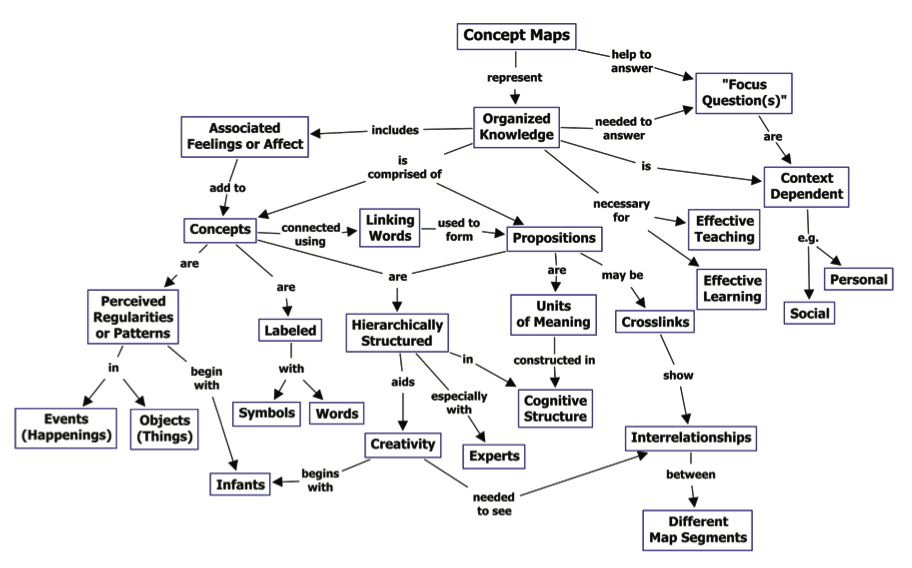
\includegraphics[width=12cm]{img/MentaleModelle/novak_concept_maps.png}
	\caption[Struktur einer Concept Map]{Struktur einer Concept Map (entnommen aus \citep[][S. 2]{Novak06})}
	\label{fig:img_MentaleModelle_novak_concept_maps}
\end{figure}

Concept Maps werden verwendet, um exploratives Lernen zu unterstützen. In diesem Fall bilden Individuen die ihnen bewussten Zusammenhänge der Realität in der Concept Map ab und erschließen bei der individuellen oder kooperativen Erstellung den Problembereich vollständiger, was zur Entwicklung eines umfassenderen Verständnisses beiträgt. Nach \citet{Novak06} können Concept Maps auch verwendet werden, um (implizites) Expertenwissen abzubilden (die Autoren beziehen sich hier auf die „Wissenspirale“ nach \citet{Nonaka95}. Im Wesentlichen ermöglichen Concept Maps damit das Externalisieren sowohl von Laien- als auch Expertenmodellen im Sinne von \citet{Seel91} und unterstützen auch die Weiterentwicklung von Laienmodellen hin zu ausgereifteren Erklärungs- oder Expertenmodellen.  Damit ist eine grundsätzliche Eignung für den Einsatz im Rahmen von auf der Externalisierung von Modellen basierender „Articulation Work“ gegeben.

\subsubsection{Vorgehen}

\citet{Novak06} schlagen vor, bei der Konstruktion einer Concept Map mit der Festlegung einer Fokus-Frage zu beginnen. Die Fokus-Frage muss klar formuliert sein und spezifisch auf das Problem oder den Sachverhalt eingehen, der in der Concept Map repräsentiert werden soll. Die Fokus-Frage dient nicht nur der Festlegung des Gegenstands der Concept Map sondern auch deren Abgrenzung nach außen (d.h. dass die Frage so spezifisch sein muss, dass Abweichungen vom intendierten Gegenstand der Concept Map erkannt werden können).

Im nächsten Schritt werden die relevanten Konzepte gesammelt. \citet{Novak06} sprechen von 15-25 Konzepten, die im ersten Durchlauf maximal verwendet werden sollten. Diese Konzepte können grob entsprechend ihrer Abstraktheit vorsortiert werden, um die Erstellung der Concept Map im nächsten Schritt zu erleichtern.

Die vorläufige Concept Map, die im nächsten Schritt erstellt wird, basiert auf den hierarchischen Zusammenhängen zwischen den gesammelten Konzepten. Zwischen diesen wird in der Folge nach „cross-links“ gesucht. Alle identifizierten Beziehungen müssen benannt werden. Im Zuge dieser ersten Herstellung von Beziehungen ergeben sich im Normalfall weitere Konzepte, die in die Concept Map aufgenommen werden müssen. Dies erfolgt im Zuge eines erneuten Durchlaufs durch den beschriebenen Prozess. Nach \citet{Novak06} benötigt eine Concept Map mindestens drei dieser Durchläufe, um ausreichende Qualität erreichen zu können.

\subsubsection{Unterstützung}

\citet{Novak06} erwähnen, dass Concept Mapping mittels Haftnotizen auf Papier oder Whiteboards durchgeführt werden kann, empfehlen aber, ein rechnerbasiertes Werkzeug -- die CMapTools \citep{Canas04} -- einzusetzen, dass den Erstellungsprozess unterstützt und den Umgang mit der entstehenden Komplexität erleichtert.

Dieses Werkzeug ermöglicht neben der Unterstützung des Mapping-Prozesses (d.h. der Nachverfolgung des Prozesses und der Möglichkeit, einzelne Schritte rückgängig zu machen) auch eine erweiterte Abbildung der Concept Map selbst. Diese umfasst unter anderem auch die Einbindung von externen Ressourcen (Dateien am Rechner), was von \citet{Novak06} als Wesentlich zur Einbettung der Concept Map in den Kontext des Problemumfelds angesehen wird.

\subsubsection{Bewertung}

Concept Mapping ist ein Ansatz zur computer-basierten Strukturierung und Visualisierung von Konzept-Netzwerken \citep{Novak06}. Durch die Rechnerunterstützung ergeben sich Vorteile hinsichtlich der Flexibilität der Darstellung und der Archivierung der Modelle. Konzeptuell werden wie bei Strukturlegetechniken Begriffsnetzwerke gebildet, wobei die methodische Hinterlegung bei Concept Mapping Ansätzen nicht so variantenreich und detailliert ausgeführt ist. 

Durch die digitale Repräsentation ist eine Concept Map leichter ohne Konsequenzen zu manipulieren, da Änderungen jederzeit rückgängig gemacht werden können. Dies ermöglicht Experimente mit dem Modell und erlaubt dem Externalisierenden eine umfassendere Ergründung und Reflexion der Modelle. Kritisch wird jedoch die im Gegensatz zu Strukturlegetechniken fehlende Unmittelbarkeit der Externalisierung betrachtet – jeder Externalisierung-Prozess muss am Rechner umgesetzt werden und setzt damit Kompetenz im Umgang mit diesem Medium voraus. \citet[][S. 30f]{Ifenthaler06}

Für die Durchführung von „Articulation Work“ erscheinen Concept Maps durch ihre semantische Offenheit vor allem zur expliziten Unterstützung von „alignment of meaning“ (vgl. \citep{Sarini02}, beschrieben in Abschnitt \ref{sec:arten_von_articulation_work}). Bei der rechner-gestützten Durchführung von Concept Mapping ist aber die Wirkung der auf einen Benutzer ausgerichteten Benutzungsschnittstelle (Monitor sowie Maus und Tastatur) auf die Interaktion zwischen den Beteiligten zu berücksichtigen.

% subsection concept_mapping (end)

% section externalisierung_mentaler_modelle (end)

\section{Zusammenfassung} % (fold)
\label{sec:mentale_modelle_fazit}

In diesem Kapitel wurde das Konzept der „Mentalen Modelle“ eingeführt und dessen Relevanz für die Durchführung expliziter „Articulation Work“ beschrieben. In weiterer Folge wurden die Externalisierung mentaler Modelle, deren Rückwirkung auf die kognitven Prozesse der Individuen sowie Methoden zu Unterstützung des Externalisierungsvorganges beschrieben. Der Zusammenhang des Themenbereichs der „Mentalen Modelle“, deren Externalisierung und deren Einbettung in den Gesamtzusammenhang von „Articulation Work“ ist in Abbildung \ref{fig:img_MentaleModelle_ArbeitInteraktionMentaleModelle} nochmals zusammenfassend dargestellt.

\begin{figure}[htbp]
	\centering
		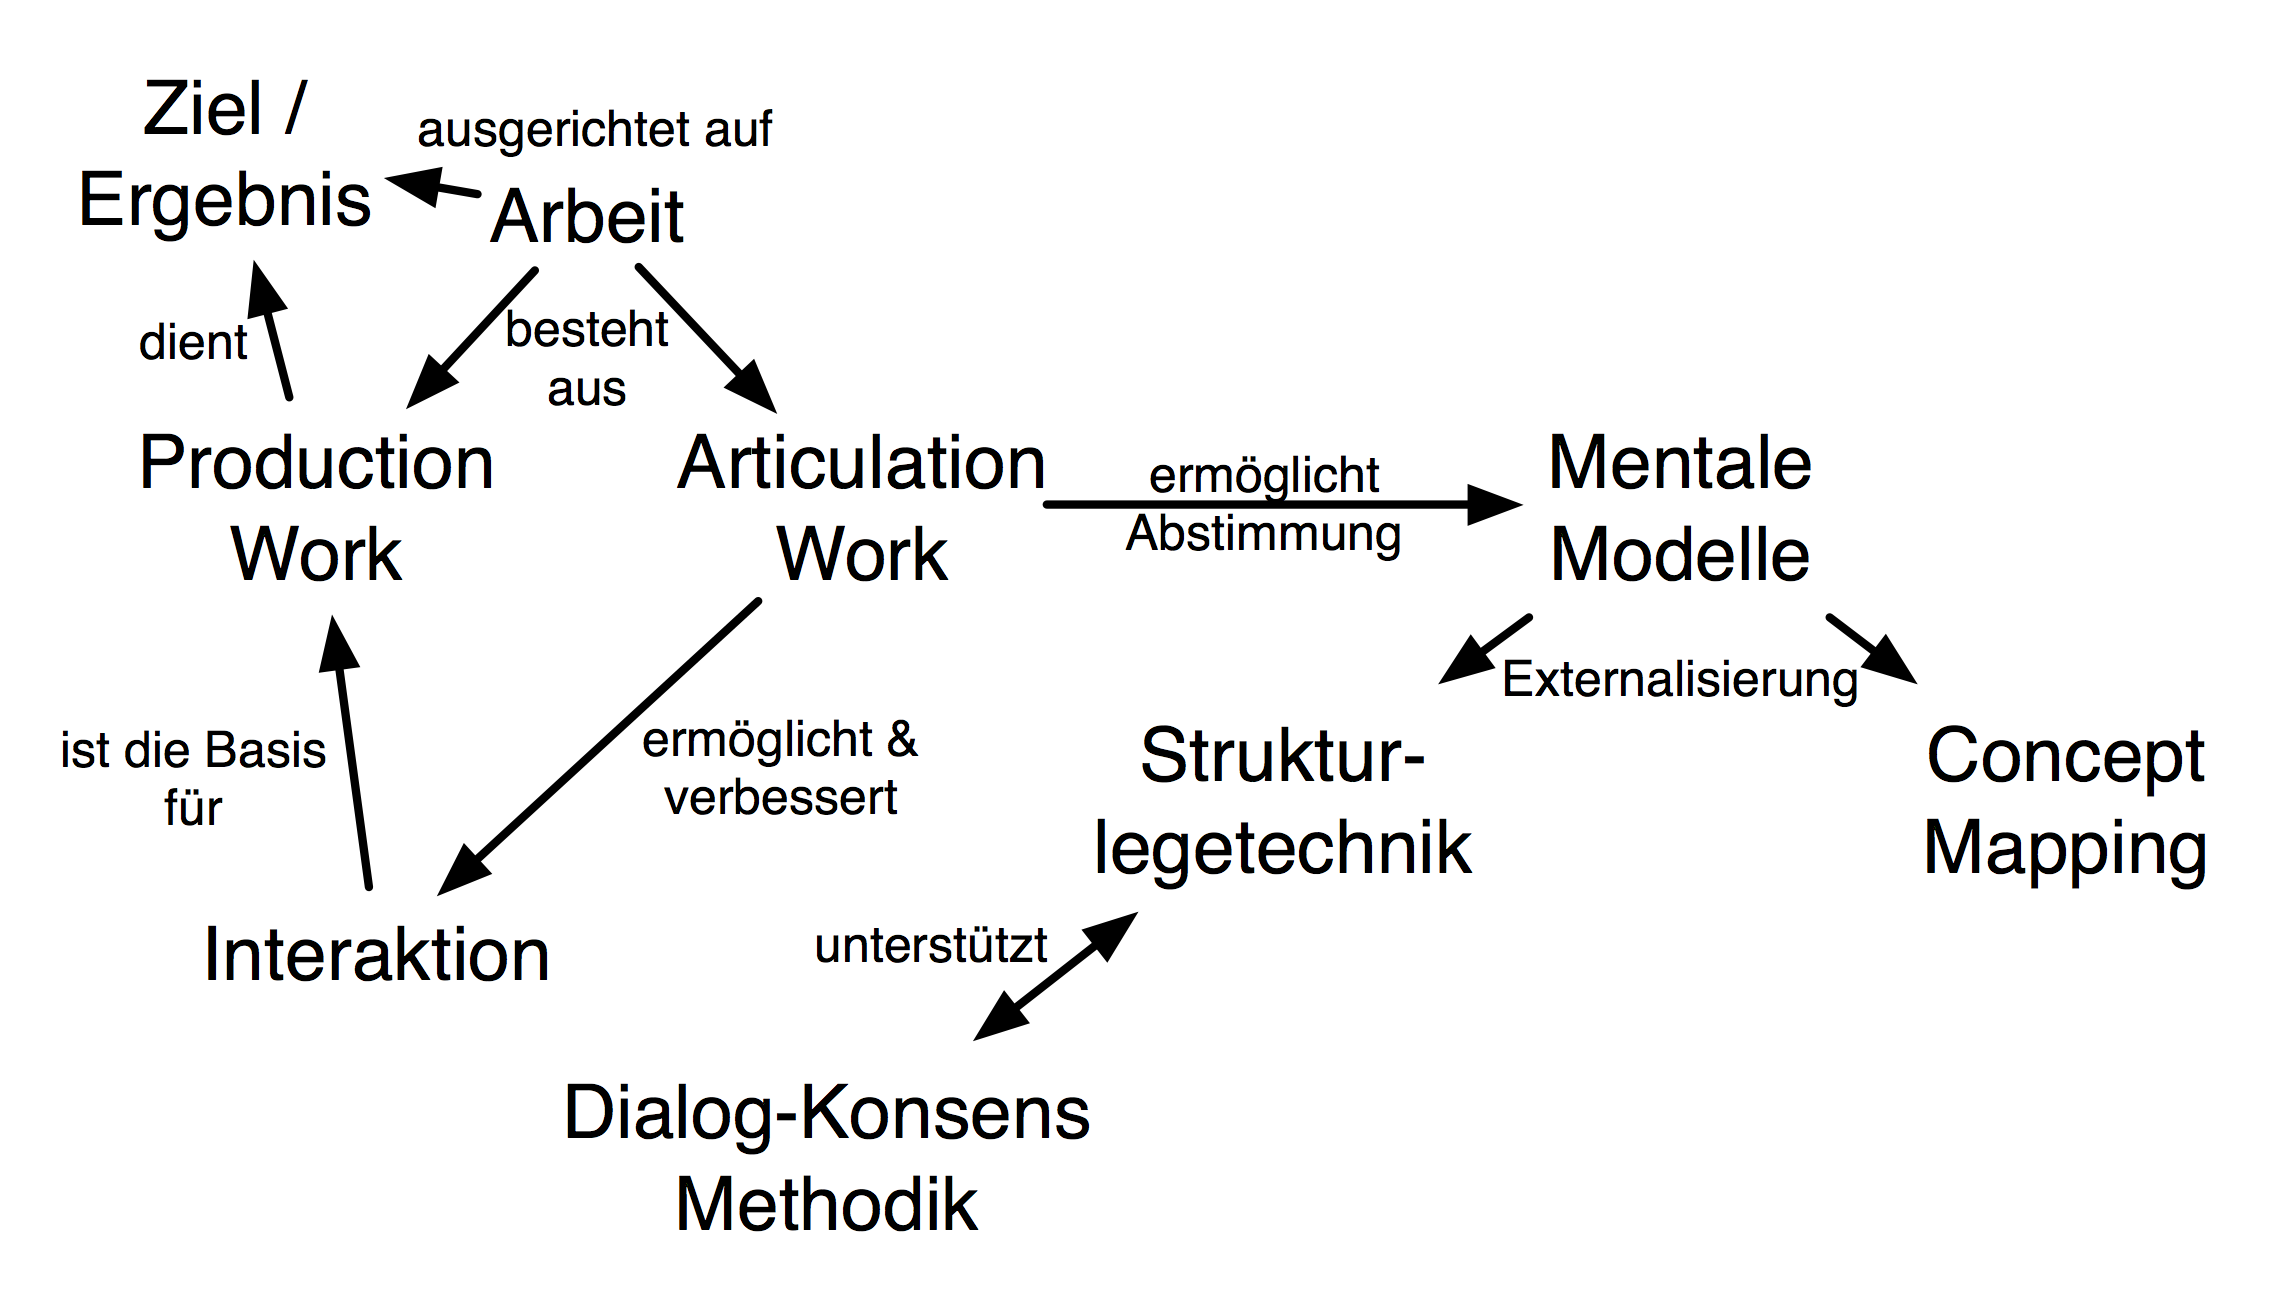
\includegraphics[width=10cm]{img/MentaleModelle/ArbeitInteraktionMentaleModelle.png}
	\caption{Mentale Modelle und Articulation Work im Gesamtzusammenhang}
	\label{fig:img_MentaleModelle_ArbeitInteraktionMentaleModelle}
\end{figure}


„Mentale Modelle“ sind ein Erklärungskonzept für jene mentalen Strukturen und Vorgänge, mit Hilfe derer Individuen ihre Wahrnehmungen der realen Welt erklären und Handlungsalternativen ableiten. Durch Lernprozesse können „Mentale Modelle“ verfeinert oder grundlegend verändert werden. Quellen für neue Information, die in mentalen Modellen abgebildet wird, können die Wahrnehmung der realen Welt, dokumentarische Ressourcen oder andere Individuen sein. Ein wesentlicher Unterstützungsfaktor für die Reflexion und Verfeinerung mentaler Modelle ist deren Externalisierung. Diese ist außerdem die Voraussetzung für die Kommunikation und Abstimmung verschiedener mentaler Modelle.

Während die Externalisierung auch rein verbal erfolgen kann, ist die Verwendung einer expliziten, graphischen Repräsentation vorteilhaft. Diese wirkt vor allem in Situationen, in denen mentale Modelle offengelegt und kommuniziert werden sollen, als Ankerpunkt und Dokumentation, anhand derer eine Abstimmung der individuellen Sichten erfolgen kann. Methoden, deren Eignung zur Externalisierung mentaler Modelle empirisch belegt ist, sind unter anderem Strukturlegetechniken und Concept Mapping. Für die im Rahmen dieser Arbeit verfolgte Unterstützung von „expliziter Articulation Work“ bieten beide Methoden Vor- und Nachteile. Deswegen wird im folgenden Kapitel eine Synthese dieser beiden Methoden angestrebt, die deren Vorteile vereint und gleichzeitig die nachteilig wirkenden Faktoren zu vermeiden sucht.

% section fazit (end)

% chapter mentale_modelle (end)

% \chapter{Mentale Modelle}
% \label{cha:mentale_modelle}
% 
% In diesem Kapitel wird das Konzept der mentalen Modelle eingeführt, das in dieser Arbeit als Erklärungsansatz für jene Aspekte von "Articulation Work" verwendet wird, die die nicht sichtbaren, kognitiven Beiträge eines beteiligten Individuums betreffen. Nach einer Einführung in die Begriffswelt der mentalen Modelle wird die Argumentation aus dem letzten Kapitel nochmals aufgegriffen und die mögliche Rolle mentaler Modelle für "Articulation Work" erörtert. In der Folge werden Methoden eingeführt mit denen mentale Modelle externalisiert und kommuniziert werden können. Basierend auf diesen Beschreibungen wird im letzten Teil des Kapitels untersucht, welche Herausforderungen sich bei der Anwendung dieser Methoden im Kontext von "Articulation Work" ergeben können.
% 
% \section{Begriffsbestimmung}e
% \label{sec:mentalemodelle_begriffsbestimmung}
% 
% Der Begriff der Mentalen Modelle wurde von \citet{Johnson-Laird81} geprägt. Ein mentales Modell ist nach 
% 
% \subsection{Mentale Modelle nach Johnson-Laird} % (fold)
% \label{sub:mentale_modelle_nach_johnson_laird}
% 
% % subsection mentale_modelle_nach_johnson_laird (end)
% 
% \subsection{Mentale Modelle nach Norman} % (fold)
% \label{sub:mentale_modelle_nach_norman}
% 
% \citet{Norman83a} formuliert ein Verständnis von mentalen Modellen aus Interaktionssicht. Sein Kontext ist die Untersuchung von Mensch-Maschine-Interaktion und den dort auftretenden Interaktionsabläufen. Mentale Modelle sind in diesem Verständnis individuelle Konstrukte, die von Menschen bei der Interaktion mit der Umwelt, mit anderen Menschen oder mit Technologie gebildet werden, um das Verhalten der Gegenseite erklären und vorhersagen zu können\footnote{\emph{„In interaction with the environment, with others, an with the artifacts of technology, people form internal, mental models of themselves and of the things with which they are interacting. These models provide predictive and explanatory power for understanding the interaction“} \citep{Norman83a}}. Um den Begriff abzugrenzen, führt \citeauthor{Norman83a} ein aus vier Elementen bestehendes Begriffssystem ein, das den Diskussionsbereich abgrenzt und definiert:
% \begin{description}
% 	\item[target system] Das Zielsystem ist jenes System, das von einer Person benutzt wird oder dessen Benutzung von dieser Person erlernt wird.
% 	\item[conceptual model of target system] Ein konzeptionelles Modell ist ein Modell, dass das Zielsystem vollständig, konsistent und exakt beschreibt. Konzeptionelle Modelle werden von Entwicklern, Designern, Wissenschaftern oder Lehrern (im Allgemeinen: Experten in der Domäne des Zielsystems) definiert.
% 	\item[mental model of target system] Mentale Modelle werden von Personen bei der Interaktion mit dem Zielsystem entwickelt, um dessen Verhalten zu erklären. Diese Modelle müssen nicht vollständig und exakt sein, müssen aber für die jeweilige Person funktional sein, d.h. für deren Zwecke ausreichendes Erklärungspotential besitzen. Mentale Modelle haben evolutionären Charakter und entwickeln sich während der Interaktion mit dem System weiter. Die Inhalte eines mentalen Modells werden durch das Vorwissen und die Erfahrung der jeweiligen Person beeinflusst.
% 	\item[scientist's conceptualization of mental model] Die Konzeptualisierung eines mentalen Modells ist der Versuch ein mentales Modell mit wissenschaftlichen Mitteln zu erheben und abzubilden. Sie soll die Inhalte des mentalen Modells möglichst vollständig und genau abbilden. Die Konzeptualisierung ist also ein Modell eines Modells.
% \end{description}
% 
% Im Weiteren nennt \citeauthor{Norman83a} sechs generelle Eigenschaften von mentalen Modellen, die er aus eine Vielzahl von Beobachtungen in unterschiedlichen Kontexten ableitet:
% \begin{enumerate}
% 	\item Mentale Modelle sind unvollständig
% 	\item Mentale Modelle können von ihren Trägern nur sehr einschränkt wiedergegeben werden.
% 	\item Mentale Modell sind instabil und werden vor allem in Bereich ungenau, die Teile des Zielsystems abbilden die lange nicht benötigt wurden.
% 	\item Mentale Modelle sind nicht klar voneinander abgrenzbar -- ähnliche Gegenstände oder Situationen werden oft hinsichtlich der angewandten Interaktionsmuster verwechselt.
% 	\item Mentale Modelle sind unwissenschaftlich -- auch mentale Modelle, die inhaltlich (technisch) überflüssiges Verhalten verursachen, werden beibehalten, wenn der Aufwand der physischen Ausführung gering ist.
% 	\item Mentale Modelle sind simpel -- auch wenn eine effizientere Interaktion möglich wäre, wenn mehr Aufwand in die Planung investiert würde bzw. ein komplexeres mentales Modell zum Einsatz käme, präferieren Benutzer einfache Modelle, deren Anwendung höheren „physischen Aufwand“ mit sich bringen.
% \end{enumerate}
% 
% % subsection mentale_modelle_nach_norman (end)
% 
% \subsection{Mentale Modelle nach Senge} % (fold)
% \label{sub:mentale_modelle_nach_senge}
% 
% % subsection mentale_modelle_nach_senge (end)
% 
% \section{Veränderung mentaler Modelle}
% \label{sub:veränderung_mentaler_modelle}
% Assimilation vs. Akkommodation
% 
% \section{Mentale Modelle und Articulation Work}
% \label{sec:mentale_modelle_und_articulation_work}
% 
% Argumentation mit Wissensspirale (Nonaka \& Takeuchi)
